\documentclass[12pt]{article}
%%%%%%%%%%%%%%%%%%%%% Packages
\usepackage[utf8]{inputenc}
\usepackage{listings}
\usepackage{color}
\usepackage{geometry}
\usepackage{natbib}
\usepackage{qcircuit}
\usepackage{verbatim}
\usepackage{multicol} 
\usepackage{hyperref} 
\usepackage{url}
\usepackage{epigraph}
\usepackage{calc}


%%%%% Epigraph bullshit
\newcommand{\mytextformat}{\itshape\epigraphsize}
\newenvironment{mytext}{\mytextformat}{}
\newenvironment{mysource}{\scshape\hfill}{}
\renewcommand{\textflush}{mytext} 
\renewcommand{\sourceflush}{mysource}
\let\originalepigraph\epigraph 
\renewcommand\epigraph[2]%
   {\setlength{\epigraphwidth}{\widthof{\mytextformat#1}}\originalepigraph{#1}{#2}}


%%%%%%%%%%%%% MATHS %%%%%%%%%%%%%%%%%%%%
\usepackage{amsmath} 
\usepackage{mathtools}
\usepackage{physics}
\usepackage{amssymb}
\usepackage{array}
%%%%%%%%% FIGurES %%%%%%%%%%%%%%%%%%%%%%%%
\usepackage{textcomp}
\usepackage{graphicx}
\usepackage{caption} 
\usepackage{scrextend}
\usepackage{pgfgantt}
\usepackage{rotating}
\usepackage{subcaption}
\usepackage{float}
\usepackage{tcolorbox}
%%%%%%%%%%%%%%%%%% variables
\definecolor{codegreen}{rgb}{0,0.6,0}
\definecolor{codegray}{rgb}{0.5,0.5,0.5}
\definecolor{codepurple}{rgb}{0.58,0,0.82}
\definecolor{backcolour}{rgb}{0.95,0.95,0.92}
\definecolor{mygray}{gray}{0.95}

\lstdefinestyle{mystyle}
{backgroundcolor=\color{mygray},   
 commentstyle=\color{codegreen},
 keywordstyle=\color{blue},
 numberstyle=\tiny\color{codegray},
 stringstyle=\color{codepurple},
 basicstyle=\footnotesize,
 breakatwhitespace=false,         
 breaklines=true,                 
 captionpos=b,                    
 keepspaces=true,                 
 numbers=left,                    
 numbersep=5pt,                  
 showspaces=false,                
 showstringspaces=false,
 showtabs=false,                  
 tabsize=2}
\lstset{style=mystyle}

\usepackage{hyperref}
\hypersetup{colorlinks=true,
            citecolor=green,
            linkcolor=blue,}
\renewcommand{\equationautorefname}{Eq.}%
\renewcommand{\figureautorefname}{Fig.}%

\graphicspath{{figures/}}
\newgeometry{left=0.8in,right=0.8in,top=1in,bottom=1in} 

%%%%%%%%%%%%%%%%
\begin{document}

\title{Quantum Meta-Programming for Dummies}
    \author{Cohort 4 \\[0.5em] Quantum Engineering CDT \\ University of Bristol}
    \date{\today}
    \maketitle

%Cohort project
%%%%%%%%%%%%%%%%%%%%%%
\chapter{Preface}
This is where the preface will be
%\newpage

\tableofcontents
\newpage

%\begin{multicols*}{2}
%%%%%%%%%%%%%%%%%%%%%%%%%%
\chapter{Introduction}


\epigraph{[Quantum computation] does not merely make computer science
a branch of physics. \\ It also makes part of experimental physics into a branch of computer science}{\textit{Quantum theory, the Church-Turing principle \\ and the universal
quantum computer \\ -- David Deutsch}}

Quantum mechanics is one of the most well-tested theories in existence [REF?]. It is also one of the most unintuitive, revealing aspects of nature at nanoscopic scales which are entirely incompatible of our own experience of the world. \\

Quantum mechanics has two key facets. The first, from which the field derives its moniker, is the quantisation of properties such as charge, angular momentum, and energy. This property has already changed the world substantially over the course of the last 70 years. Among technologies such as the laser and magnetic resonant imaging (MRI), perhaps the greatest impact has been made through the manipulation of semiconductor technology. Since the invention of the first transistor in 1947 \cite{Bardeen1948}, this semiconductor technology has laid the groundwork for scalable computers, bringing us into the information age. \\

The development of this technology comes at a critical time in the conventional silicon industry. The famous Moore's law, hypothesised in its current form in 1975, stated that the number of transistors per square inch would double every two years. This law models the exponential scaling of computing power since its conception incredibly well, as we can see in \autoref{fig:Moore's_Law}. This was driven partly by the cost and power consumption per transistor going down as feature sizes decreased \cite{MooresLawEconomist}.  However, now increasingly small feature sizes have resulted in energy efficiencies and profitability are starting to plateau, while technical issues continue to increase. These issues are in part due to quantum effects such as tunnelling.  \\


\begin{figure}[h!]
	\centering
	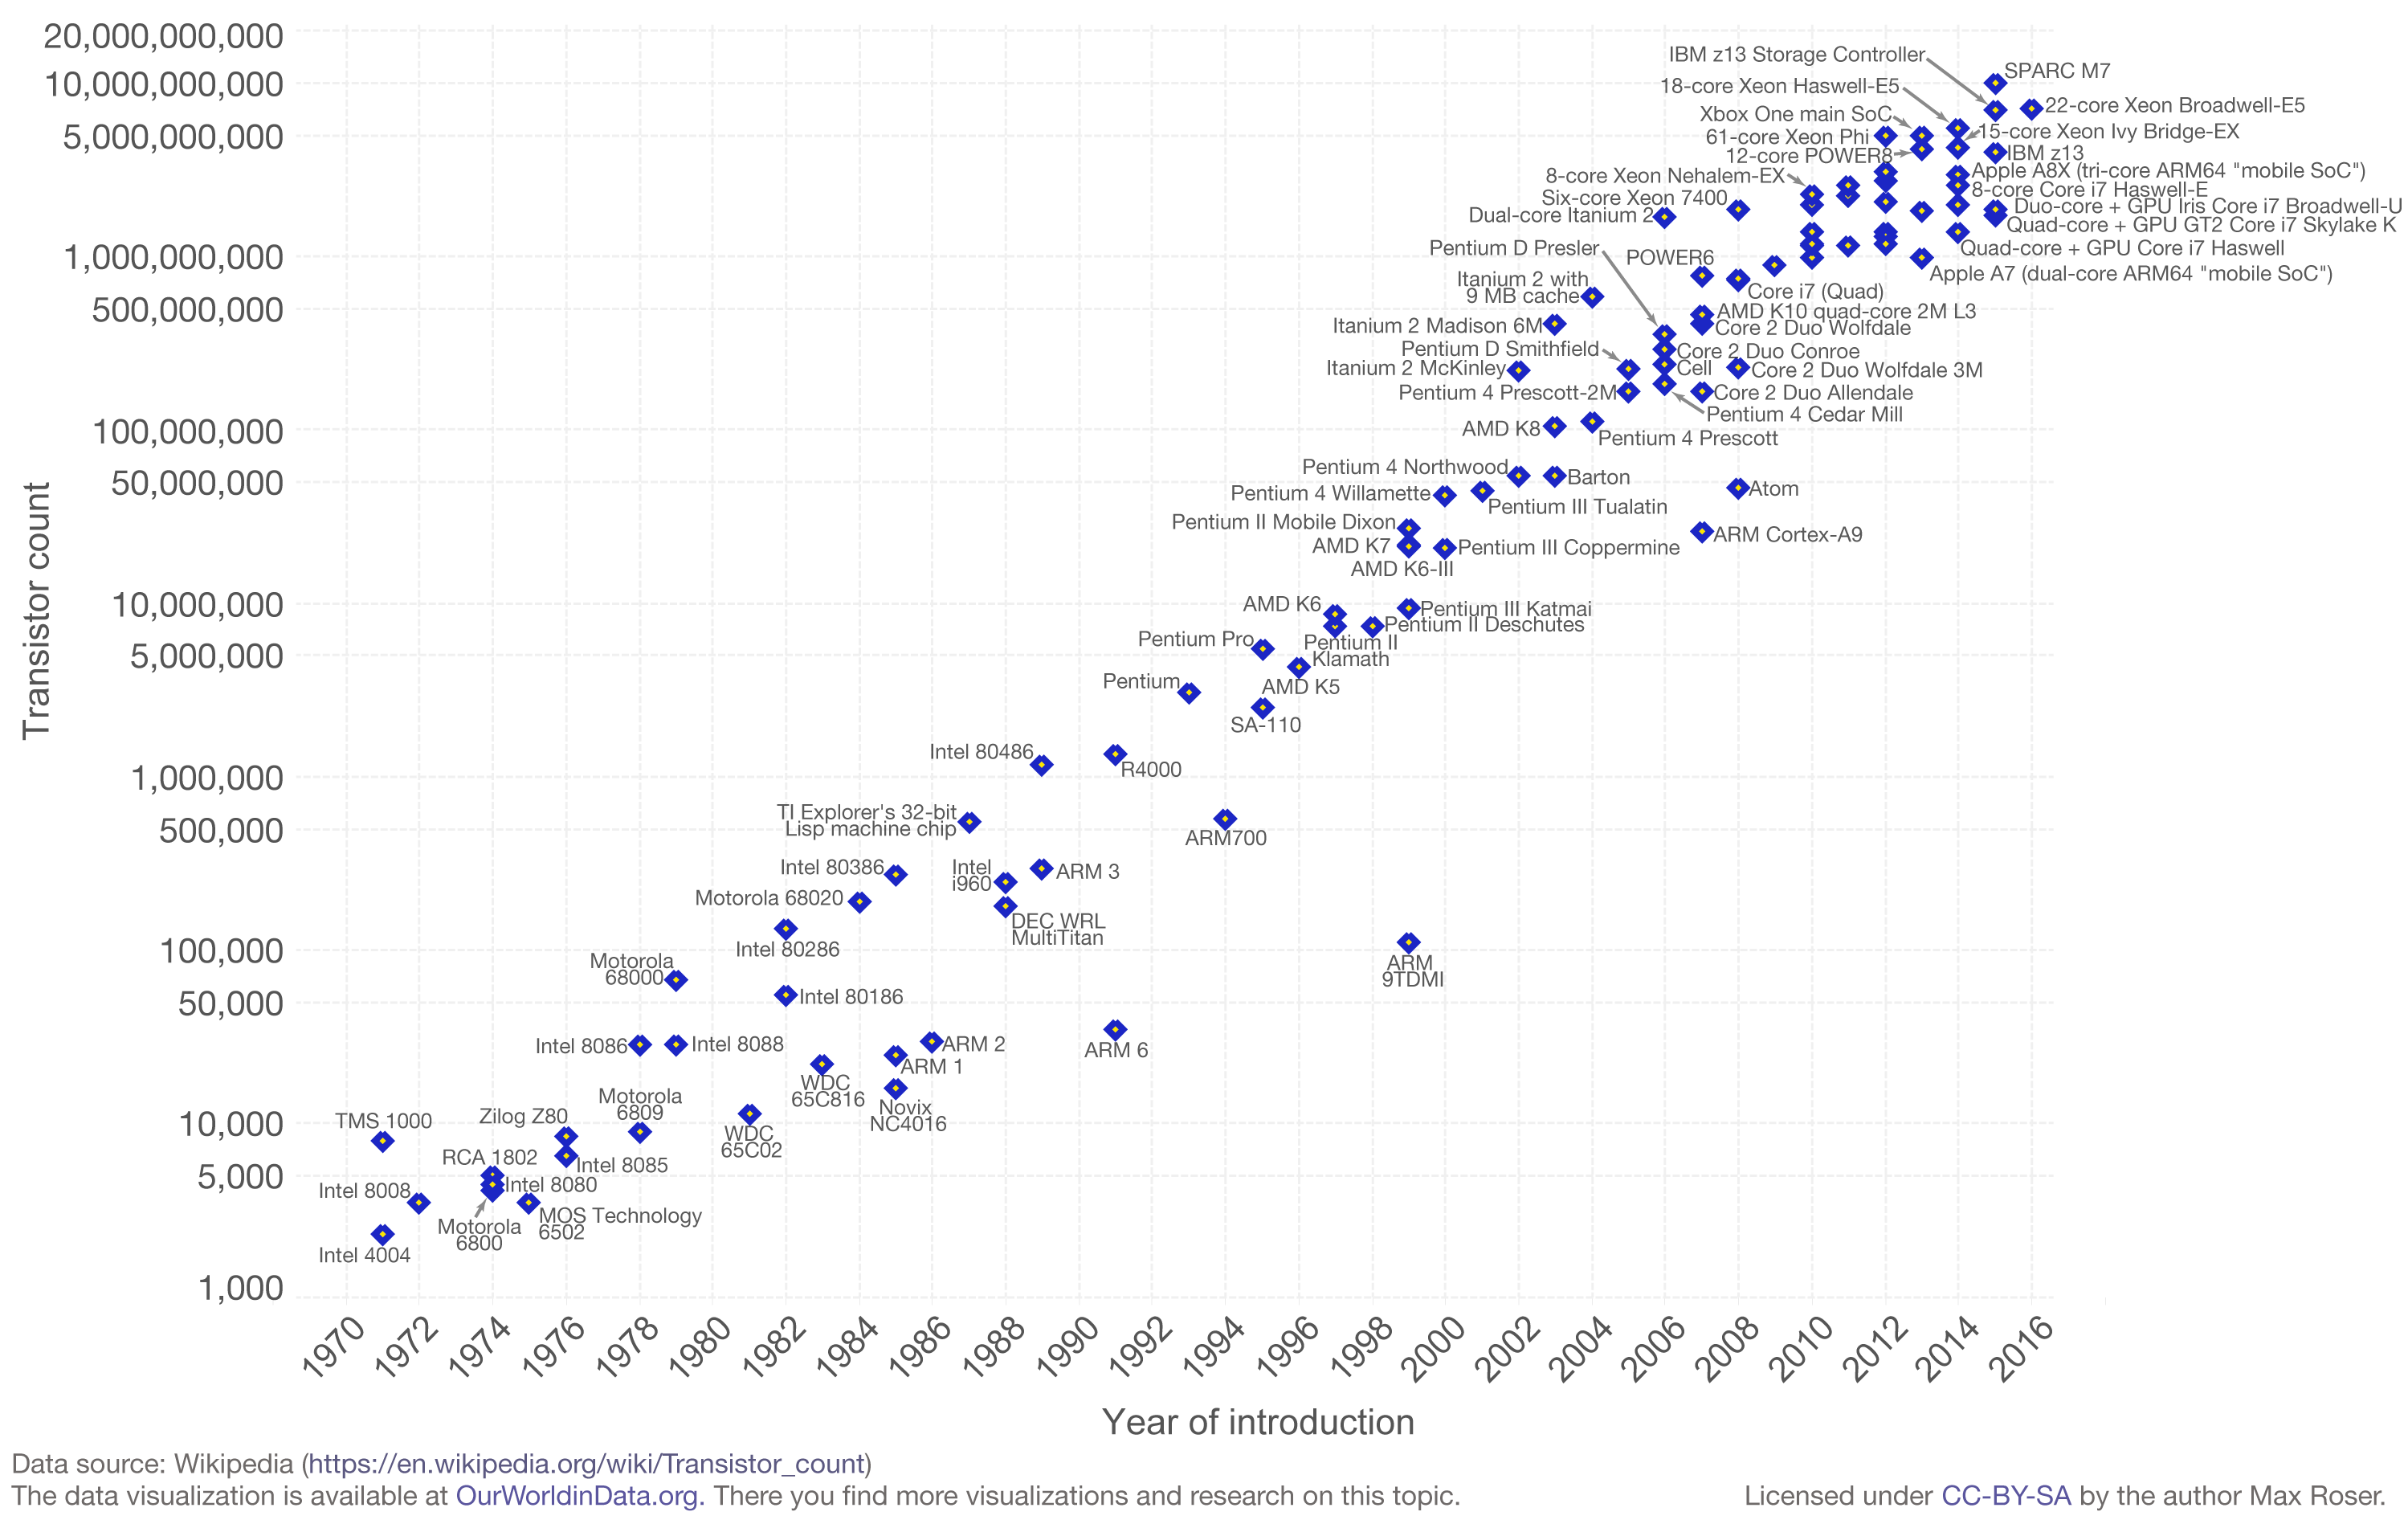
\includegraphics[width = \linewidth]{Moores_Law.png}
	\caption{Chart showing Moore's law, with a logarithmic increase in transistor 	count on each chip from 1970-2016.}
	\label{fig:Moore's_Law}
\end{figure}

This example of tunnelling is related to the so-called `wave-particle duality' which is the second key feature of quantum mechanics. Which is causing these issues may the solution in addition to the problem. The distinction between waves and particles, whose behaviour is well established in classical physics, becomes blurred. \textbf{Every object in the universe, if the correct energy and length scales are chosen, will display both of these aspects to some degree.} \\

It is in this property in which lies the tantalising promise of quantum computing. Particles like electrons, which have comprised the backbone of electricity and classical information for the past century, have the ability to behave in a wave-like manner: they could contain not just the binary bit choices of 0 or 1,  but one of an infinite number of continuous values, called `qubits'. Combined with entanglement to allow our qubits to influence each other while in this state, we can harness a sort of parallelism that results from the wave-like nature of controlled particles.  \\


While in general it is doubtful that a quantum computer will be generically  `faster' than a classical computer, and it is much harder to engineer, we do have significant potential to outperform conventional computers at certain tasks. While the amount of information processing in a conventional computer scales linearly with the number of bits, a quantum computer scales exponentially with the number of qubits for these tasks. Thus adding a single extra qubit could double the computing power. These are discussed, along with the quantum algorithms used to implement them, in Chapter \autoref{Algorithms and applications}. At the point when quantum computers are able to outperform classical supercomputers at a task, the so-called `quantum supremacy' will have been achieved. \\

These tasks range from \ldots\\ 

 

However, achieving this potential does not come without significant difficulty. Readout or detection of the information in the qubit destroys the information contained within, resulting in us reverting to the classical bit values with some probability. Furthermore, the technology is still very young and undeveloped. Algorithms exist for many of the applications above, but there may be many more as yet undiscovered. Academic institutions , large corporations (including Google \cite{bristlecone}, IBM, Intel) and small start-ups (Rigetti, \cite{rigettihome}) alike have invested heavily in hardware. There are a wide range of platforms and architectures, including but not limited to superconducting qubits \cite{bristlecone}, ion traps [REF], quantum dots [REF], spin qubits in silicon [REF], and silicon photonics [REF]. \\


One crucial area that remains comparatively underdeveloped is software. It will be crucial to provide this missing link between the theoretical algorithm and its implementation on a quantum computer. Ideally `quantum' programming should adopt many of the features as its classical counterpart: it should be usable by any person without understanding the details of the hardware being used, it 


Over the next few years and decades quantum computing is likely to become a reality. It will be crucial when this becomes the case that people are able to understand how to use these machines in order to harness their applicability to the areas of mathematics, computer science, chemistry and finance. This guide is designed to be an introduction to the science of quantum computers and the current state of the field. Initially we explain in more depth how quantum computers work and their differences to classical computers in Chapter \autoref{TheBasics}. Since in the short-term, quantum computers are likely to be noisy, error-prone and limited in scale, we discuss how they can be used in this regime in \autoref{Short term quantum computing}. \\

Once the engineering of quantum computers have been improved, then a host of more impressive applications can be demonstrated, which are considered in chapter \autoref{Algorithms and applications}. We examine the programming languages that will be able to interface between the algorithms and the quantum computer in chapter \autoref{Programming a future universal quantum computer}, and hardware-specific implementations and architectures in chapter \autoref{Implementations}. \\

A more complete description of quantum mechanics is given in chapter \autoref{Advanced Topics} for any interested party. 

%\newpage

%%%%%%%%%%%%%%%%%%%%%%%%%%%%%%
\section{Weird Vector things}\label{TheBasics}
The fundamental unit of information in classical computing is the bit. which takes one of two states usually represented with 0 or 1. Modern silicon chips realise this as the `on' or `off' state of a transistor. In an analogy with bits, the fundamental unit for quantum computing is the qubit. The represents the simplest, fully quantum system 

\begin{lstlisting}[language=Python]
vec = [a,b]
\end{lstlisting}
%\newpage

%%%%%%%%%%%%%%%%%%%%%%%%%%%
\section{Quantum Circuits}

This section briefly reviews the gate model for circuit based quantum computing and discusses the similarities between between digital and quantum computers. The gate model is one of the most popular architectures for quantum computation at the moment. \textit{Intel \cite{intelqcomp} IBM \cite{ibmqweb}, Google \cite{googleqai}, Rigetti \cite{rigetti}} \textbf{REF!} are all using the gate model approach for quantum computing.

Both forms of computation follow the same structure, you start with bits (or qubits), operations are performed on the (qu)bits and then you measure the new values of the (qu)bits. We show an example in \autoref{fig:basicoperation}.

%%%% digital circuit
\begin{figure}[H] 
\centering
\begin{subfigure}[h]{0.4\textwidth}
\begin{align*}
\Qcircuit @C=0.5cm @R=0.7cm
{&\lstick{A} &\multigate{2}{Operation} & \\
&\lstick{B} &\ghost{Operation} & \\
&& &\qw &\lstick{Q} \\}
\end{align*}
\caption{Digital operation}
\label{fig:digitalcirc}
\end{subfigure}
~
%%%% Q circuit
\begin{subfigure}[H]{0.4\textwidth}
\begin{align*}
\Qcircuit @C=0.5cm @R=0.7cm
{&\lstick{A} &\multigate{2}{Operation} &\qw &\lstick{A} \\
&\lstick{B} &\ghost{Operation} &\qw &\lstick{B} \\
&\lstick{Q} &\ghost{Operation} &\qw &\lstick{Q} \\}
\end{align*}
\caption{Quantum operation}
\label{fig:quantumcirc}
\end{subfigure}
\caption{resource flow}
\label{fig:basicoperation}
\end{figure}

This  

\subsubsection{Digital logic}

Every digital computing operation can be built up from NAND logic gates \cite{sheffer1913set}. We call this a universal gate for computation.

\begin{figure}[h]
  \centering
  \begin{subfigure}[h]{0.4\textwidth}
  \centering
  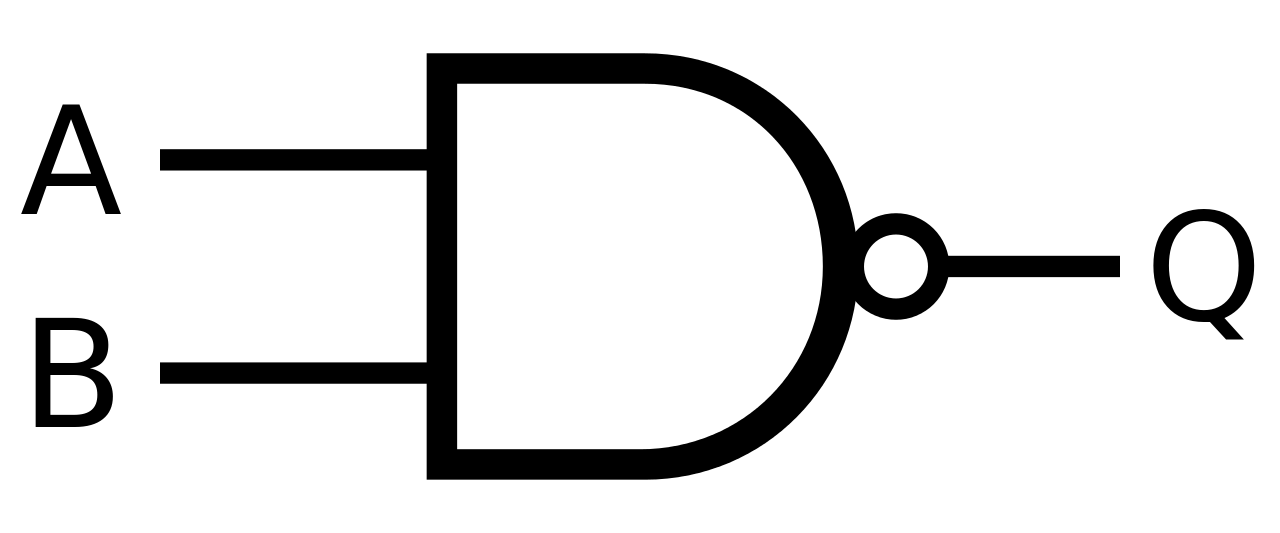
\includegraphics[width=0.7\textwidth]{NAND_ANSI_Labelled_svg.png}
  \caption{The NAND logic gate \cite{nandwiki}.}
  \label{fig:NAND}
\end{subfigure}
~
  \begin{subfigure}[h]{0.4\textwidth}
  \centering
  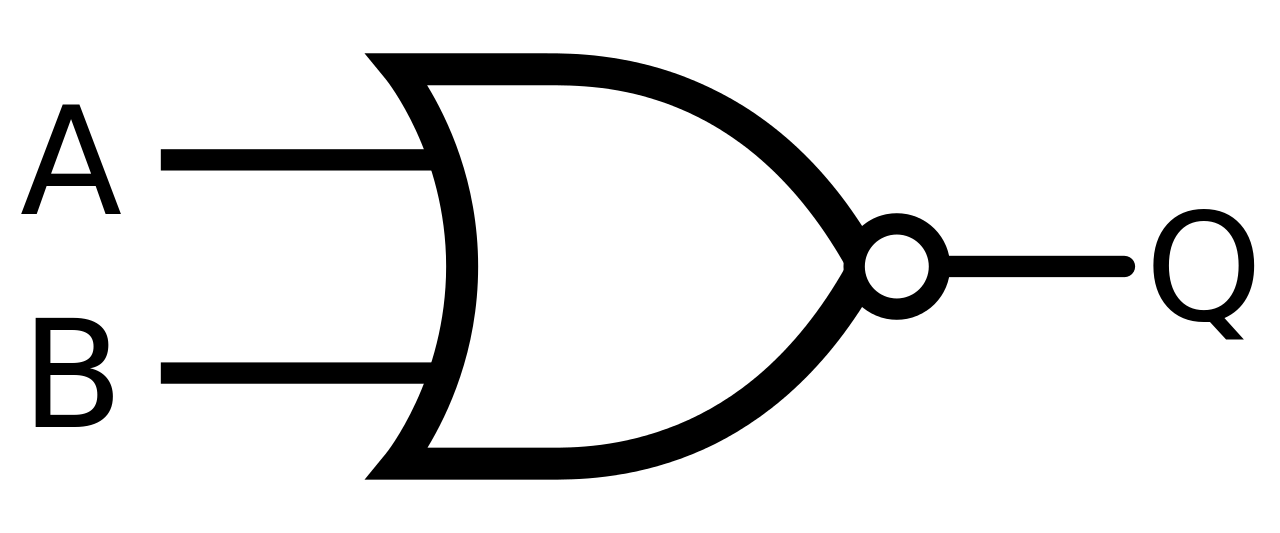
\includegraphics[width=0.7\textwidth]{NOR_ANSI_Labelled_svg.png}
  \caption{The NOR logic gate \cite{norwiki}.}
  \label{fig:NOR}
  \end{subfigure}
\end{figure}

reversible logic

%%%%%%%%% circuit 1 
\begin{figure}[h!]
\begin{align*}
\Qcircuit @C=0.5cm @R=0.7cm
{%1
&\lstick{S_1} &\gate{H} &\ctrl{1} &\qw \\
%0
&\lstick{S_0} &\ctrl{-1} &\targ &\qw \\}
\end{align*}
\caption{Schur transform for 2 qubits}
\label{cir:vanilla2}
\end{figure}


\newpage

%%%%%%%%%%%%%%%%%%%%%%%%%%%%%%%%%%%%

%%%%%%%%%%%%%%%%%%%%%%%%%%%%%%%%%%%%%
\section{Short term quantum computing}\label{Shortqcomp}
In this section we aim to give a comprehensive overview of quantum computing platforms which are currently available and discuss the near-term advantages that these platforms can bring.

%%%%%%%%%%%%%%%%%%%%%%%%%%%%%%%%%%%%%%%%%%%%%%%%%%%%%%%%%%%%%%%
\subsection{Adiabatic quantum computing \& quantum annealers}
Dwave, NISC
QUBO problems.

Quantum Algorithms in Dwave? optimisation? Quantum Monte Carlo speed-up? Simulating quantum systems

%%%%%%%%%%%%%%%%%%%%%%%%%%
%%%%%%%%%%%%%%%%%%%%%%%%%%
\subsection{Rigetti- Forest}

%\subsubsection{pyQuil}

Rigetti has created an environment called Forest, amongst its contributions is a python library called PyQuil. With PyQuil one can simulate up to 26 qubits on the Quantum Virtual Machine (QVM). An example code from \cite{rigetti} is detailed below with comments to assist the reader:
\begin{lstlisting}[language=Python]
from pyquil.quil import Program
from pyquil.gates import H, CNOT
from pyquil.api import SyncConnection
# construct a Bell State program
p = Program()
p.inst(H(0))
p.inst(CNOT(0, 1))
# run the program on a QVM
qvm = SyncConnection()
result = qvm.wavefunction(p) 
# produces the output wavefunction of the Bell state
\end{lstlisting}
Rigetti also offers access to a 19 qubit processor they call 19Q. This API 
\begin{lstlisting}[language=Python]
import numpy as np
 
def incmatrix(genl1,genl2):
    m = len(genl1)
    n = len(genl2)
    M = None #to become the incidence matrix
    VT = np.zeros((n*m,1), int)  #dummy variable
 
    #compute the bitwise xor matrix
    M1 = bitxormatrix(genl1)
    M2 = np.triu(bitxormatrix(genl2),1) 
 
    for i in range(m-1):
        for j in range(i+1, m):
            [r,c] = np.where(M2 == M1[i,j])
            for k in range(len(r)):
                VT[(i)*n + r[k]] = 1;
                VT[(i)*n + c[k]] = 1;
                VT[(j)*n + r[k]] = 1;
                VT[(j)*n + c[k]] = 1;
 
                if M is None:
                    M = np.copy(VT)
                else:
                    M = np.concatenate((M, VT), 1)
 
                VT = np.zeros((n*m,1), int)
 
    return M
\end{lstlisting}

\subsubsection{Example Codes}

% \subsubsection{Language} 5

%%%%%%%%%%%%%%%%%%%%%%%%%
%%%%%%%%%%%%%%%%%%%%%%%%%
\subsection{IBM- Project Q}
IBM has launched the IBM Q experience that consists of a development environment called QISkit and a higher-level gate-building platform that allows users to compose their own algorithms. The devices used to perform the simulation and computation are based on a superconducting charge qubit implementation, which can be found described in more detail in \autoref{Implementations}.  This development environment is also based on python, as we saw with Forest by rigetti. There is ample space for development of algorithms in this environment as the visual arrays provide a clear structure to those familiar with quantum computation. The composer also displays the code on which it operates so that users interested in further development have the opportunity to learn how to code their own gates in QISkit. The associated documentation which is linked on the IBM Q website provides more detail to the structure \cite{coles2018quantum}. Updates are regularly posted to the main site. Additional features such as limited access to a larger register of bits are available to academics. Specifications of the device that is being used to perform these calculations are available on the website as seen in \autoref{fig:ibmsite}. 

\begin{figure}[h!]
\centering
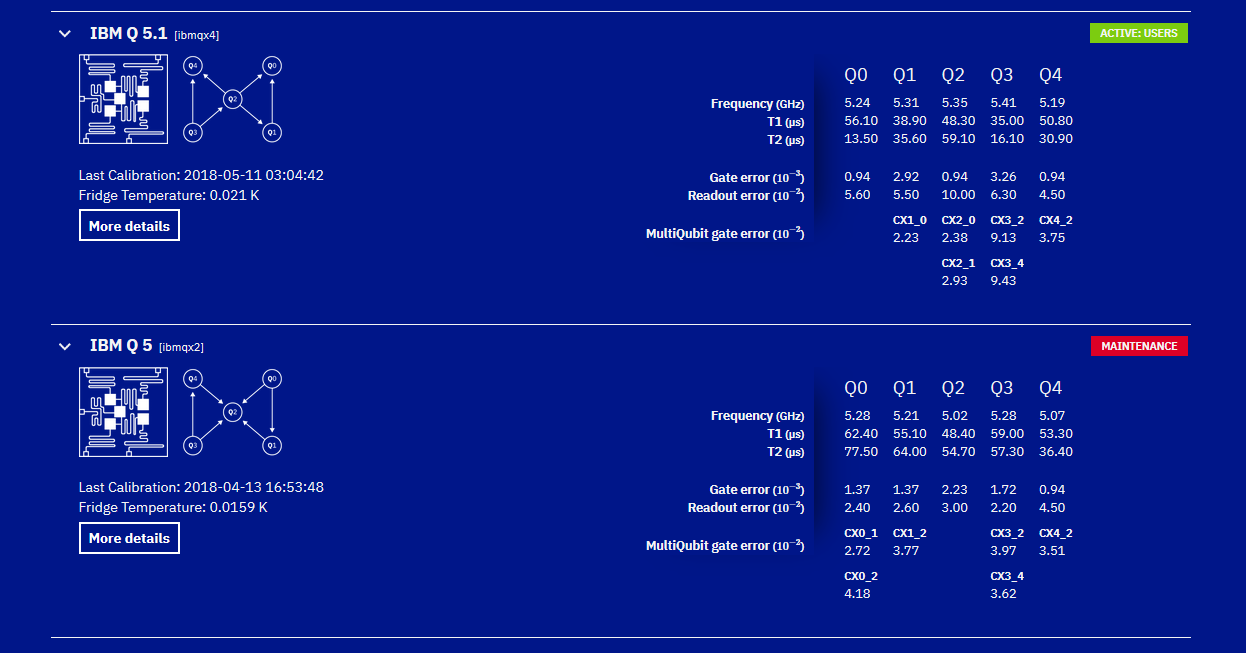
\includegraphics[width=12cm]{ibmsite}
\caption{The description of the devices used for the IBM Q suite as of early May 2018 (must be updated closer to submission). Cooling refrigerator temperature along with the update structure is presented. A useful live display feed allows users to track both the physical and computational side of their own algorithms made on the composer.}
\label{fig:ibmsite}
\end{figure}

\subsubsection{Example Codes}
Examples of composed codes in this environment are based on adding sequences of pre-defined gates. An example of two single-qubit operations being performed on bit 0 out of the 0-4 register.  
\begin{figure}[h!]
\centering
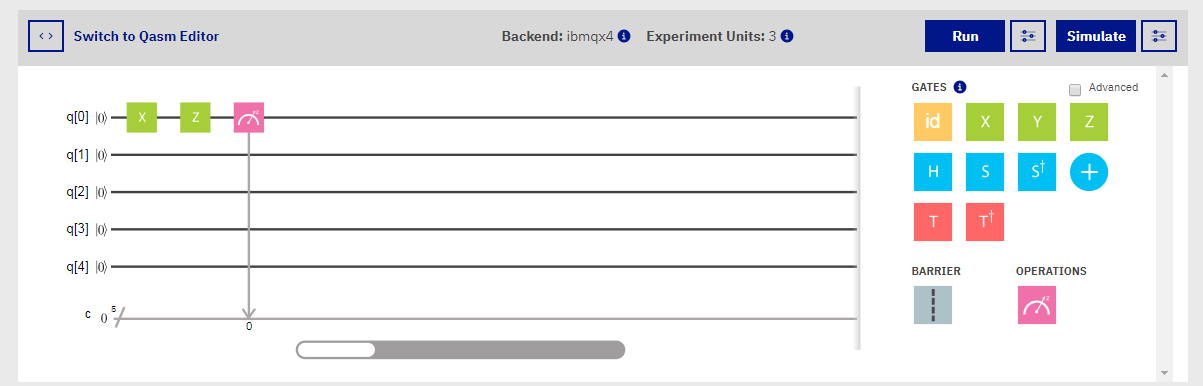
\includegraphics[width=10cm]{IBMq_1}
\caption{An example of the composition suite that allows gates to be strung together. In this instance, the first qubit in the register has the X and Z gates performed on it before measurement. The symbolism is identical to the standard gate model used within this guide, which makes the transition from other environments simpler.}
\end{figure}
%\begin{figure}
%\centering
%\includegraphics[width=10cm]{IBMq_2}
%\caption{In this example, the composition consists of building a set of gates that }
%\end{figure}

\newpage

%%%%%%%%%%%%%%%%%%%%%%%%%%%%%%%
\chapter{Algorithms and applications}\label{Algorithmsandapplications}

We now discuss the three primary types of algorithms that take advantage of a quantum computer.

%%%%%%%%%%%%%%%%%%%%%%%%%%%%%%%%%%%%%%%
\section{Quantum transforms}
1
\subsection{Quantum Fourier transform}
2
\subsection{Schur transform}
3
%%%%%%%%%%%%%%%%%%%%%%%%%%%%%%%%%%%%%%%%%
\section{Number theory algorithms}
4
\subsection{Shor's algorithm}
5
\subsection{Discrete Logarithm problem}
6
%%%%%%%%%%%%%%%%%%%%%%%%%%%%%%%%%%%%%%%
\section{Oracular algorithms}
7
\subsection{Grover's algorithm}
Grover's algorithm solves the unstructured search problem in $O(\sqrt[]{N})$ queries \cite{Grover1996,Grover1997} compared to average number of $O(N)$ queries required for classical algorithms. Although Grover's algorithm does not allow quantum computers to solve NP-complete problems in polynomial time, it does provide a quadratic speedup over classical algorithms. Grover's algorithm is based on the principle of selective phase-shifting on one state (which satisfies a certain condition) of a quantum system at each iteration. A simple case of Grover's algorithm for $ N = 2^n$ elements with exactly one marked element has been described in the following box:
\begin{tcolorbox}
We are given access to $f: \left\{0,1\right\}^n \rightarrow \left\{0,1\right\}$ with the promise that $f(x_0) = 1$ for a unique element $x_0$. We use a quantum circuit on $n$ qubits with initial state $\ket{0}^{\otimes n}$.  Let $H$ denote the Hadamard gate, and let $U_0$ denote the $n$-qubit operation which inverts the phase of $\ket{0^n}$: $U_0\ket{0^n} = -\ket{0^n}$, $U_0\ket{x} = \ket{x}$ for all $x \neq 0^n$.
\begin{enumerate}
\item Apply $H^{\otimes n}$.

\item Repeat the following operations T times, for some T to be determined later:
\begin{enumerate}
\item Apply $U_f$, where $U_f\ket{x} = (-1)^{f(x)}\ket{x}$.
\item Apply $D$, where $D = -H^{\otimes n}U_0H^{\otimes n}$
\end{enumerate} 
\item Measure all the qubits and output the result.
\end{enumerate}
\end{tcolorbox}

In circuit diagram form, Grover's algorithm appears like:
\begin{equation*}
\Qcircuit @C=1.14em @R=1.25em
{\lstick{\ket{0}} & \gate{H} & \multigate{5}{U_f} & \multigate{5}{D} & \multigate{5}{U_f} & \ghost{U_f} & \lstick{\dots} & \multigate{5}{D} & \meter \\
\lstick{\ket{0}} & \gate{H} & \ghost{U_f} & \ghost{D} & \ghost{U_f} & \ghost{U_f} &\lstick{\dots} & \ghost{D} & \meter \\ 
& \dot{} & & & & & & & \dot{} \\
& \dot{} & & & & & & & \dot{} \\
& \dot{} & & & & & & & \dot{} \\
\lstick{\ket{0}} & \gate{H} & \ghost{U_f} & \ghost{D} & \ghost{U_f} & \ghost{U_f} & \lstick{\dots} & \ghost{D} & \meter \\}
\end{equation*}


\subsection*{Circuit complexity}
In Grover's algorithm, gates $U_f$ and $D$ are applied on the qubits repeatedly until the desired state is found. It is the underlying hardware of these two gates that decide the intrinsic cost of Grover's algorithm per iteration \cite{Matthew2017}. This means that the total time complexity of Grover's algorithm is the number of iterations ($O(\sqrt[]{N})$) multiplied by the ``overhead" provided by the gates $U_f$ and $D$. The hardware construction of gate $U_f$ depends upon the problem being solved by the algorithm while the hardware for gate $D$ is independent of the problem and only depends upon the number of qubits required by the algorithm. 
\subsubsection{Construction of gate $D$}
The gate $D$ for $n$-qubits can be implemented in the following manner. This shows that gate $D$ requires $2n+1$ Hadamard ($H$) gates, $2n+1$ Pauli $X$ gates and an n-control Toffoli gate.

\begin{align*}
\Qcircuit @C=1.14em @R=1.25em
{\lstick{\ket{x_1}} & \gate{H} & \gate{X} &  \ctrl{1} & \gate{X} & \gate{H} & \qw  \\
\lstick{\ket{x_2}} & \gate{H} & \gate{X} &  \ctrl{4} & \gate{X} & \gate{H} & \qw  \\
\lstick{\dot{}} & \dot{} & \dot{} & & \dot{} & \dot{} & \\
\lstick{\dot{}} & \dot{} & \dot{} & & \dot{} & \dot{} & \\
\lstick{\dot{}} & \dot{} & \dot{} & & \dot{} & \dot{} & \\
\lstick{\ket{x_n}} & \gate{H} & \gate{X} &  \ctrl{1} & \gate{X} & \gate{H} & \qw  \\
\lstick{\ket{0}} & \gate{x} & \gate{H} &  \targ & \qw & \qw & \qw }
\end{align*}

\subsubsection{Construction of gate $U_f$}
The action of $U_f$ on qubits is defined as,
\begin{equation}
U_f\ket{x} = (-1)^{f(x)}\ket{x}
\end{equation}
Therefore, the underlying hardware of $U_f$ depends upon the function, $f(x)$.
\subsubsection{The hidden subgroup problem}
9
%%%%%%%%%%%%%%%%%%%%%%%%%%%%%%%%%%%%%%%
\section{Approximations \& Simulating quantum systems}
10
\subsection{Approximating Matrix powers}
11
\subsection{Approximating Partition functions}
12

%\newpage

%%%%%%%%%%%%%%%%%%%%%%%%%%%%%%%%%%%%
\chapter{Programming a future universal quantum computer}\label{Programmingquantumcomputer}
Three languages will be covered here: Q\#, Quil and Scaffold.
\section{Implementing Shor's algorithm}
2
\subsubsection{Language 1}
3
\subsubsection{Language 2}
4
%%%%%%%%%%%%%%%%%%%%%%%%%%%%%%%%%%%%
\section{Implementing Grover's algorithm}
5
\subsubsection{Language 1}
6
\subsubsection{Language 2}
7
%%%%%%%%%%%%%%%%%%%%%%%%%%%%%%%%%%%
\section{Implementing the matrix power approximation}
8
\subsubsection{Language 1}
9
\subsubsection{Language 2}
10
%%%%%%%%%%%%%%%%%%%%%%%%%%%%%%%%%
\section{Language features}
11
\subsubsection{Language 1}
12

%%%%%%%%%%%%%%%%%%%%%%%%%%%%%%%%%%
\section{The universal quantum computer}
13

%\newpage

%%%%%%%%%%%%%%%%%%%%%%%%
\chapter{Implementations}\label{Implementations}

--- PLAN ---

Focus on implementation of quantum programming languages

Implementing quantum computers:
\begin{itemize}
\item Comparison of quantum and classical computer architectures
Classical computer architectures: ALU, CPU, buses, memory, instructions, etc equivalents for quantum computers? Quantum architectures: gates? Cluster states? Quantum vs. Classical control? What are the analogues of instructions, execution, buses and memory? Are there fundamental limits to architecture design (imposed by eg no cloning. Does memory make sense in the same way as for classical computers? Quantum memory is more like single-use working-registers). How about classical computers with quantum instructions? What about qbranch instructions?   
\item Different quantum computing platforms 
Probably just a few -- maybe linear optical quantum computers and iron traps. 
\item Classical language compilers
\end{itemize}
Implementing quantum programming:
\begin{itemize}
\item Quantum error correction
Not entirely analogous to classical computers, (no instruction execution errors). Can error correction be abstracted away from the compiler level? Would error correction take place at the equivalent level of (say) instruction pipe lining in a classical processor?    
\item Quantum language compilers
What is the quantum equivalent of object code? Does it contain machine code (instructions to be executed, analogous to classical computers) or does it compile into an arrangement of gates, or some other computation mode (measurements in a cluster state?). The architecture of the quantum computer would probably heavily inform the structure of low level languages. (For example, C has basic structures essentially based on mov, branch, and arithmetic and bit manipulation instructions). Hence the low level languages of gate based quantum computers will be based on structures easily realised using gates (the gates themselves, presumably analogous to bit manipulation; coherent arithmetic, (implemented using gate arrangements lifted from half and full adders); flow control -- presumably classical; and strict mov operations, ie excluding copy). Low level languages targeted at cluster state implementation will have cluster state measurements as primitive operations (equivalent to bit manipulation) in the language, and presumably various other generic operations (like control, branching, etc.) What kind of optimisations does the C compiler do, and what are the equivalents in the quantum cases? 
\end{itemize}
--- PLAN ---

\section{Computer architecture and programming languages}
\subsection{Classical computer architecture}
\subsection{Low level classical languages}
\subsection{Compilers and abstraction}
\section{Quantum computer architectures}
\subsection{Overview}
\subsection{What are the qubits?}
\subsection{What are the operations?}
\subsection{Putting it all together}
\section{Comparison of classical and quantum architectures}
\section{Low level quantum programming languages}
\section{Quantum compilers and high level languages}
\section{The future}

%\newpage

%%%%%%%%%%%%%%%%%%%%%%%%%%%%
\section{Advanced topics}\label{Advancedtopics}
1
%%%%%%%%%%%%%%%%%%%%%%%%%%%%%%%
\subsection{Quantum mechanics: The basics}

In this section we cover some supplementary background quantum theory. Although a deeper knowledge of quantum theory would serve to further your understanding of quantum computing, it should not be necessary for sections 1 to 7. You have seen in Section (?) that the state of a system governed by quantum mechanics can be represented by a binary 1 or 0, similar to that of a classical bit. However this is not the only two options. In general the state of a bit can now be in a superposition of both 1 and 0, collapsing to one or the other when measured. In this section we will cement this description into a more formal language that will help you to probe deeper into more advanced literature.

\subsubsection{Quantum States}

In quantum mechanics, we describe the state of a system simply with labels. These labels we assign to the system, such as {`0',`1'}, aim to give some intuition about the state of the system. We could equally have used {`open', `closed'} if we were trying to describe the state of a door. Formally these labels are called quantum numbers and in general are not restricted to be one of two values.\\

For example, imagine the 4 of spades was chosen from a deck of cards, a good choice of label to describe the card would be `4' or `spade'. Equally in a quantum system we would say that the card is in the state `4' or `spade' which we write formally as $\ket{4}$, or $\ket{spade}$. In this scenario the quantum number `4' could have been one of 13 values, therefore the set of states needed to fully describing the system are $\{\ket{A}, \ket{2}, \ket{3},\ldots ,\ket{K}\}$ with quantum numbers $\{A,2,3,\ldots K\}$. If the set of quantum numbers are unique and their associated states describe all possible values a properties can take then they are said to form a Hilbert space $\mathcal{H}$ of the system. Formally we say the set of independent and orthonormal states span a Hilbert space:

\begin{equation}
\mathcal{H}:=span\{\ket{A}, \ket{2}, \ket{3},\ldots ,\ket{K}\}
\end{equation}

The Hilbert space should loosely be thought of as a vector space. It's purpose is to mathematically define all the possible states a system can be in. This is a very useful tool when we start to describe the evolution of a system because it has better be the case that our description of a system remains physically possible. For example, it would make no sense to talk about the state $\ket{A}$ evolving to the state $\ket{spade}$. In that sense, the Hilbert space helps define the boundaries of your system.\\

The notation $\ket{\ldots}$ is called a `ket' and for every `ket' there is a `bra' written as $\bra{\ldots}$. The names originates from the first and second halves of the word `braket', which when placed together resemble the most important operation in quantum computation: the inner product. The inner product is a simple function that does the following:\\

\textit{if state $\ket{a}$ is the same as state $\ket{b}$ return 1 else return 0}\\

In quantum physics notation this operation is performed by turning the ket $\ket{a}$ into a bra, $\bra{a}$. The `bra' $\bra{a}$ and `ket' $\ket{b}$ are then used to form the word `braket' and is equal to 1 or 0 depending on whether the state a is equal to the state b.\\

For example, returning to our deck of cards, the inner product of the states $\ket{A}$ with $\ket{5}$ is written as:

\begin{equation}
\bra{A}\ket{5} = 0
\end{equation}

Conversely, the inner product of the states $\ket{J}$ with $\ket{J}$ would be:

\begin{equation}
\bra{J}\ket{J} = 1
\end{equation}

When a set of state are unique in this way, they are said to be orthonormal. The inner product is important as it allows you to check that all the state that form your Hilbert space are orthonormal and will become very useful when we introduce superposition in the next section.

\subsubsection{Superposition}

In quantum mechanics, using the states that form the basis of our Hilbert space to describe the system is not enough. Observation of quantum systems tell us that when we prepare a state multiple times and measure it, the outcome will not always be the same. At this point its crucial to point out that the formalism does not try to explain why this is the case, but only provides a way of describing the system. I highlight this fact for the following reason. Typically when confronted with a new phenomena, we turn to the mathematical description to gain some intuition of its causes. With quantum mechanics, the formal description should not be used to find a "logical" explanation of how superposition works but only to help fully describe the observed physics of the system.\\

To understand how we can describe this phenomena formally, lets make our deck of cards a quantum deck of cards that now obeys the laws of quantum mechanics and see how we can reflect our observations within the maths.\\

The first thing to note is that the act of measurement appears to perform an operation on the system that takes it from its superposition state to a basis state of the Hilbert space.

For example, lets say you are given a face down card that when flipped multiple times is sometimes a queen and sometimes a 4. Before performing the operation of turning it over the state of the card should be thought of as being in a superposition of $\ket{Q}$ and $\ket{4}$. Only under the operation of flipping it does it become one of the two basis states. Repeating many times would allow us to build up a picture of the probabilities of getting either one of the other. Since all we have to describe the system pre-measurement are the probabilities of getting each state after measurement, this is what we will use.\\

Formally, given a state $\ket{\psi}$ that is said to be in superposition of the states $\ket{a}$ and $\ket{b}$ where the probability of getting the state $\ket{a}$ is $\abs{\alpha}^{2}$ and the probability of getting the state $\ket{b}$ is $\abs{\beta}^{2}$ then we describe the state as:

\begin{equation}
\ket{\psi} = \alpha \ket{a} + \beta \ket{b}
\end{equation}

In general, both $\alpha$ and $\beta$ can take complex values and so to ensure that the probabilities are real we take the absolute value squared. The significance of having complex values will be discussed later on but for now its sufficient to consider them as real.\\

Returning to our example, say we get a queen one third of the time and a four two thirds of the time. We would describe the pre-measurement state as:

\begin{equation}
\ket{\psi} = \frac{1}{\sqrt{3}} \ket{Q} + \frac{2}{\sqrt{6}}  \ket{4}
\end{equation}

where

\begin{equation}
\abs{\frac{1}{\sqrt{3}}}^{2}+ \abs{\frac{2}{\sqrt{6}}}^{2} =1
\end{equation}

as expected since the probabilities of getting a queen or a four must sum to one. Consider a more general case where the state is in a superposition over all possible state in the Hilbert space. Lets call this state $\ket{\phi}$ and it is given by:

\begin{equation}
\ket{\phi} = \sum_{i=0}^{n} c_{i}\ket{\phi_{i}}
\label{equation:bigphi}
\end{equation}

% Superposition is a property of the physical object (in this case the card) which manifests itself under a measurement operation.\\


% Unlike classical representations, quantum states can be formed from superpositions of the computational basis elements of the form $|\psi\rangle = \alpha |0\rangle + \beta |1\rangle$. Taking the inner product allows us to evaluate the probability of measuring a result $\braket{\psi} = |\alpha|^{2} \braket{0}+|\beta|^{2}\braket{1}$. $\alpha$ and $\beta$ represent the weighting of the states they precede, hence P$_{0}=|\alpha|^{2}$ and P$_{1}=|\beta|^{2}$. In general, states may be formed of an arbitrarily long superposition of basis states $\ket{\phi_{n}}$, as in the example given in \ref{equation:bigphi}.

% \begin{equation}
% \ket{\Phi} = \sum_{0}^{n} c_{n}\ket{\phi_{n}}
% \label{equation:bigphi}
% \end{equation}
% where the coefficients $c_{n}$ must satisfy $\sum |c_{n}|^{2} = 1$ which can be understood as all outcome probabilities $P_{n}=|c_{n}|^{2}$ must sum to one. 
\subsubsection{Entanglement}
4 
\subsubsection{Errors \& Decoherence}
5 
%%%%%%%%%%%%%%%%%%%%%%%%%%%%%%%%
\subsection{Error correcting codes}
6
\subsection{}

%\newpage

%%%%%%%%%%%%%%%%%%%%%%%%%%%%%%%%%%%%%%%%%
\begin{verbatim}
https://github.com/ot561/qprogramming/tree/master
\end{verbatim}

\bibliographystyle{unsrt}
\bibliography{References}

%\end{multicols*}
\end{document}
